\chapter{Background}

This chapter concludes the fundamental knowledge that is needed to comprehend the upcoming practical work. Firstly, an introduction to cloud computing will be held. Next, a throrough understanding of honeypots is given. Lastly, we introduce some concepts of intrusion detection systens.

\section{Virtualization}

\subsection{Docker}

\section{Cloud Computing}\todo{Check cites}

Nowadays it is one of the well-known keywords and has been used by vary large companies such as Google, or Amazon, however, the term \enquote{cloud computing} dates back to the late 1996, when a small group of technology executives of Compaq Computer framed new business ideas around the Internet.\cite{regalado2020} Starting from 2007 cloud computing evolved into a serious competitor and outnumbered the keywords \enquote{virtualization}, and \enquote{grid computing} reported by Google trends \cite{Wang2010}. Shortly, various cloud provider become publicly available, each with their own strengths and weaknesses. For example IBM's Cloud\footnote{\url{https://www.ibm.com/cloud}}, Amazon Web Services\footnote{\url{https://aws.amazon.com/}}, and Google Cloud\footnote{\url{https://cloud.google.com/}}. Why are clouds so attractive in practice?

\begin{itemize}
    \item It offers major advantages in terms of cost and reliability. When demand is needed, consumers do not have to invest in hardware when launching new services. Pay-as-you-go allows flexibility.
    \item Consumer can easily scale with demand. When more computational resources are required due to more requests, scaling up instances in conjunction with a suited price model are straightforward.
    \item Geographically distributed capabilities supply the need for world-wide scattered services.
\end{itemize}

In this section, we want to give basic unterstandings of cloud computing. First, we exhibit the history and draw some motivation. Following, we look at some the definitions, and point out characteristics. Lastly, we give an short introduction to HeiCloud, a cloud service that is offered by Heidelberg University.

\subsection{Definition of Cloud Computing}

Considering the definition of Brian Hayes, cloud computing is \enquote{a shift in the geography of computation} \cite{hayes2008}. Thus, computational workload is moved away from local instances towards services and datacenters that provide the need of users \cite{Armbrust2010}.

Considering the definition of the \ac{nist}, cloud computing \enquote{is a model for enabling ubiquitous, convenient, on-demand network access to a shared pool of configurable computing resources (e.g., networks, servers, storage, applications, and services) that can be rapidly provisioned and released with minimal management effort or service provider interaction} \cite{Mell2011}. \ac{nist} not only reflects the geographical shift of resources such as datacenters, but also mentions on-demand usage that contributes to a flexible resource management. Morever, \ac{nist} composes the term in five essential characteristics, three service models (see \autoref{subsec:cloud-service}), and four deployment models (see \autoref{subsec:cloud-deployment}) \cite{Mell2011}:\\

\textit{On-demand-self-service} refers to the unilaterally provision computing capabilities. Consumers can acquire server time and network storage on demand without a human interaction.\\

\textit{Broad network access} characterizes the access of capabilities of the network through standard protocols such as \ac{http}. Heterogeneous thin and thick client platforms should be supported.\\

\textit{Resource pooling} allows the provider's computing resources to be pooled across several consumers. A multi-tanent model with different physical and virtual resources are assigned on demand. Other aspects such as location are independent and cannot be controlled on a low-level by consumers. Moreover, high-level access to specify continent, state, or datacenter can be available.\\

\textit{Rapid elasticity} offers consumers to extend and release capabilities easily. Further automization to quickly increase resources  when demand skyrockets significantly can be supported regardless limit and quantity at any time.\\

\textit{Measured service} handles resources in an automated and optimized manner. It uses additional metering capabilities to trace storage, processing, bandwith, and active user accounts. This helps to monitor, and control resource usage. Thus, contributing to transparency between provider and consumer.

\subsection{Service models}
\label{subsec:cloud-service}

Service models are categorized by \ac{nist} into three basic models based on usage and abstraction level. \autoref{fig:cloud-functionalities}\todo{Fix image} shows the connection between each model whereas cloud resource are defined in \autoref{subsec:cloud-deployment}. Due to vast range of functionalities, \ac*{iaas} builds the foundation of service models. Each model on top represents a user-friendly abstraction with derated capabilities. \autoref{tab:example-service-models} shows examples of such service models.

\begin{figure}[h]
    \centering
    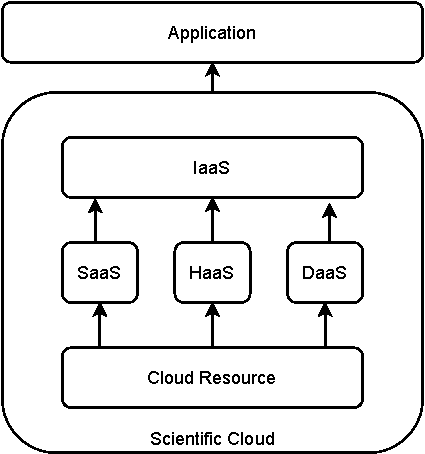
\includegraphics[width=0.4\textwidth]{figures/cloud-functionalities.pdf}
    \caption{Cloud functionalities (derived from \cite{Wang2010})}
    \label{fig:cloud-functionalities}
\end{figure}

\ac{saas} is a high-level abstraction to consumers. Controlling the underlying infrastructure is not supported. Often provider uses a multi-tenancy system architecture to organize each consumer's application in a separate environment. It helps to employ scaling with respect to speed, security availability, disaster recovery, and maintenance. Main objective of \ac{saas} is to host consumer's software or application that can be accessed over the Internet using either a thin or rich client.\cite{Dillon2010} \enquote{Limited user-specific application configuration settings} can be made \cite{Mell2011}.\\

\ac{paas} pivots on the full \enquote{Software Lifecycle} of an application whereas \ac{saas} distincts on hosting complete applications. \ac{paas} offers ongoing development and includes programming environment, tools, configuration management, and other services. In addition, the underlying infrastructure is not managed by the consumer.\\

\ac{iaas} offers a low-level abstraction to consumers with the ability to run arbitrary software regardless of operating system or application. In contrast to \ac{saas}, IT infrastructures capabilities (such as storage, networks) can be used. It strongly depends on virtualization due to integration, or decomposition of physical resources. \\

\ac{daas} serves as a virtualized data storage service on demand. Motivations behind such services could be upfront costs of on-premise enterprise database systems.\cite{Dillon2010} Mostly they require \enquote{dedicated server, software license, post-delivery services, and in-house IT maintenance} \cite{Dillon2010}. Whereas \ac{daas} costs solely what consumer's need.When dealing with a tremendous amount of data, file systems and RDBMS often lack in performance. \ac{daas} outruns such weak links by employing a table-style abstraction that can be scaled.\cite{Dillon2010}\\

\ac{haas} offers IT hardware, or datacenters to buy as a pay-as-you-go subscription service. The term dates back to 2006 during a time when hardware virtualization became more powerful. It is flexible, scalable and manageable.\cite{Wang2010}\\

\begin{table}[h]
    \centering
    \caption{Examples for cloud service models}
    \begin{tabularx}{\linewidth}{X|X|X|X|X}
        SaaS            & PaaS                  & IaaS       & Daas             & HaaS       \\ \hline
        Google Mail     & Google App Engine     & HeiCloud   & Adobe Buzzword   & Amazon EC2 \\
        Google Docs     & Windows Azure         & Amazon EC2 & ElasticDrive     & Nimbus     \\
        Microsoft Drive & AWS Elastic Beanstalk &            & Google Big Table & Enomalism  \\
                        &                       &            & Amazon S3        & Eucalyptus \\
                        &                       &            & Apache HBase     &            \\
    \end{tabularx}
    \label{tab:example-service-models}
\end{table}

\subsection{Deployment models}
\label{subsec:cloud-deployment}

Deployment models are categorized by \ac{nist} into four basic models. Each differs in data privacy, location, and manageablility \cite{Mell2011}. \autoref{tab:example-deployment-models} shows examples of such deployment models.

\begin{table}[h]
    \centering
    \caption{Examples for cloud deployment models}
    \begin{tabular}{l|l|l|l}
        Private Cloud & Community Cloud & Hybrid Cloud & Public Cloud     \\ \hline
                      & Seafile         &              & Amazon EC2       \\
                      & Nextcloud       &              & Google AppEngine \\
    \end{tabular}
    \label{tab:example-deployment-models}
\end{table}

Private clouds offer the highest level of control in regard of data privacy, and utilization. Mostly, such clouds are deployed within in a single organization, either managed by in-house teams or third party suppliers. In addition, it can be on or off premise. Within private clouds consumers have full control of their data. Especially for European data privacy laws, it is not negligible when data is stored abroad and thus under law of foreign countries. However, the popularity has not been withdrawn due to immense costs when moving towards public clouds. \cite{Dillon2010} \cite{Mell2011}\\

Community clouds can be seen as a conglomerate of mutliple organizations that merge their infrastructure with respect to a commonly defined policy, terms, and condition beforehand.\\

Public clouds represents the most used deployment models. In contradiction to private one, public clouds are fully owned by the service provider such as business, academics, or government organization. Consumers do not know where their data is distributed. In addition, contracts underlie custom policies.\\

Hybrid cloud is a mixure of two or more cloud infrastructures, such as private and public cloud.However, each entity keeps its core element. However, hybrid clouds defines \enquote{standardized or propriertary technology to enables data and application portability}\cite{Mell2011}.\\

\section{Honeypots}

The term \enquote{honeypot} exists since more than a decade. 1997 was the first time that a free honeypot solution became public. \ac{dtk}, developed by Fred Cohen, released the first honeypot solution. However, the earliest drafts of honeypots are from 1990/91, and built the foundation for Fred Cohen's \ac*{dtk}. Clifford Stoll's book \enquote{The Cuckoo's Egg}\cite{stroll2000}, and Bill Cheswick's whitepaper \enquote{An Evening With Berferd}\cite{Cheswick92} describe concepts that are consider nowadays as honeypots.\cite{Spitzner2003} A honeypot itself is a security instrument that collects information on buzzing attacks. It disguises itself as a system, or application with weaklinks, so that it gets exploited and gathers knowledge about the adversary. In 2002 a Solaris honeypot helped to detect an unknown dtspcd exploit. Interestingly, a year before in 2001 the Coordination Center of \ac{cert}, \enquote{an expert group that handles computer security incidents}\todo{citation}, shared their concerns regarding the dtspcd. Communities were aware that the service could be exploited to get access and remotely compromise any Unix system. However, during this time such an exploit was not known, and experts did not expect any in the near future. Gladly, early instances based on honeypot technologies could detect new exploits and avoid further incidents. Such events lay emphasis on the importance of honeypots.

\subsection{Definition of a Honeypot}

Dozen of defintions for honeypots circulate through the web that causes confusion, and misunderstandings. In general, the objective of a honeypot is to gather information about attacks, or attack patterns \cite{NawrockiWSKS2016}. Thus, contributing as an additional source of security measure. See \autoref{subsec:honeypot-security-concept} for a detailed view regarding honeypots in the security concept. As Spitzner et al. \cite{Spitzner2003} has listed, most misleading defintions are: honeypot is a tool for deception, it is a weapon to lure adversaries, or a part of an intrusion detection system. In order to get a basic understanding, we want to exhibit some of the key definitions. Spitzner et al. \cite{Spitzner2003} defines honeypots as a \enquote{security resource whose value lies in being probed, attacked, or compromised}. Independent of its source (e.g. server, application, or router), we expect that our instance is getting probed, attacked, and eventually exploited. If a honeypot does not match this behaviour, it will not provide any value. It is important to mention that honeypots do not have any production value, thus, any communication that is acquired is suspicious by nature \cite{Spitzner2003}. In addition, Spitzner et al. points out that honeypots are not bounded to solve a single problem, hence, they function as a generic perimeter, and fit into different situation. Such functions are attack detection, capturing automated attacks, or alert/warning generator. An example 

\begin{figure}[h]
    \centering
    \begin{tikzpicture}
  % = = = = = = = = = = = = = = = =
  % servers
  % = = = = = = = = = = = = = = = =
  \node[server](server 1){};
  \node[server, right of= server 1](server 2){};
  \node[server, right of= server 2](server 3){};

  \node[rack switch, above of=server 2,xshift=0.1cm,yshift=0.3cm]
  (rack switch 1){};

  \draw[thick,darkgray!10!gray] (server 1.north)--(rack switch 1);
  \draw[thick,darkgray!10!gray] (server 2.north)--(rack switch 1);
  \draw[thick,darkgray!10!gray] (server 3.north)--(rack switch 1);

  \begin{scope}[xshift=3.5cm]
    \node[server](server 4){};
    \node[server, right of= server 4](server 5){};
    \node[server, right of= server 5](server 6){};

    \node[rack switch, above of=server 5,xshift=0.1cm,yshift=0.3cm]
    (rack switch 2){};

    \draw[thick,darkgray!10!gray] (server 4.north)--(rack switch 2);
    \draw[thick,darkgray!10!gray] (server 5.north)--(rack switch 2);
    \draw[thick,darkgray!10!gray] (server 6.north)--(rack switch 2);
  \end{scope}

  % = = = = = = = = = = = = = = = =
  % switch
  % = = = = = = = = = = = = = = = =
  \node[yshift=1cm, l3 switch, above of =rack switch 1](l3 switch 1){};
  \node[yshift=1cm, l3 switch, above of =rack switch 2](l3 switch 2){};

  \begin{scope}
    \draw[thick,darkgray!10!gray] (rack switch 2.north)--(l3 switch 2);
    \draw[thick,darkgray!10!gray] (rack switch 1.north)--(l3 switch 1);
  \end{scope}
  
  \begin{scope}
    \node[xshift=1.7cm, yshift=1cm,scale=0.2, above of = l3 switch 1] (brouter) {\router{}} 
      edge[very thick,darkgray!10!gray] ([xshift=0.1cm,yshift=0.5cm]l3 switch 1)
      edge[very thick,darkgray!10!gray] ([xshift=0.1cm,yshift=0.5cm]l3 switch 2);
    \node[yshift=0.65cm,my cloud, minimum width=1.25cm, minimum height=1.55cm, above of = brouter, font=\large] (it) {Internet} edge[very thick,darkgray!30!gray] (brouter);
  \end{scope}
  
  % = = = = = = = = = = = = = = = =
  % Labels
  % = = = = = = = = = = = = = = = =
  \node[xshift=1.5cm,right of = brouter,align=right](lev5) {Gateway Router};
  \node[xshift=0.5cm, right of = rack switch 1,align=right](lev1) {DMZ};
  \node[xshift=0.5cm, right of = rack switch 2,align=right](lev2) {Internal};

  % = = = = = = = = = = = = = = = =
  % paths
  % = = = = = = = = = = = = = = = =
  \draw[stealth-stealth,very thick, red!80!black,shorten <=0.025cm,
  shorten >=0.56cm]([yshift=-0.25cm]brouter.west)--
  ([xshift=0.05cm]l3 switch 1.north);

  \draw[stealth-stealth,very thick, red!80!black,shorten <=0.025cm,
  shorten >=0.56cm]([yshift=-0.25cm]l3 switch 1.south)--
  ([xshift=0.05cm]rack switch 1.north);
\end{tikzpicture}
    \caption{Example of honeypots in a simplified network (derived from \cite{Spitzner2003})}
    \label{fig:honeypot-example}
\end{figure}

In general, we differentiate two types of honeypots
\begin{enumerate*}[label=(\roman*)]
    \item Production honeypots
    \item Research honeypots
\end{enumerate*}. This categorization has their origin from Mark Rosch developer of Snort during his work at GTE Internetworking.\\

Production honeypots are the common type of honeypots everyone would think of it. The objective is to protect production environments, and to mitigate the risk of attacks. Normally, production honeypots are easy to deploy within an organization. Mostly, low-interaction honeypots are chosen due to a significant reduce in risk. Thus, adversaries might not be able to exploit honeypots to attack other systems. Downside is a lack of information. Standard information like the origin of attacks, or what exploits are used can be collected, whereas insides about communication of attackers, or deployment of such attacks are unlikely to obtain. In contrast, research honeypots do fulfill this objective.\cite{Spitzner2003}\\

Research honeypots are used to learn more in detail about attacks. The objective is to collect information about the clandestine organizations, new tools for attacks, or the origin of attacks. Research honeypots are unlikely for production environments due to a higher increase of risk. Facing an increase in deployment complexity, and maintenance does not attract a production usage.\cite{Spitzner2003}\\

It is worth to mention that there is no exact line between research or production honeypots. A possible cases are honeypots that could function as either an production or an research honeypot. Due to their dynamic range in which they are applicable it makes it hard to distinguish.\\

Provos et al. adds an additional differentiation for the virtual honeypot framework \cite{Provos2003} and splits it into the following types:

\begin{itemize}
    \item Physical honeypots are \enquote{real machines on the network with its own IP address} \cite{Provos2003}
    \item Virtual honeypots are \enquote{simulated by another machine that responds to network traffix sent to the virtual honeypot} \cite{Provos2003}
\end{itemize}

\subsection{Level of Interaction}
\label{subsec:interaction-honeypots}

When building and deploying a honeypot, the depth of information has to be defined beforehand. Should it gather unauthorized activities, such as an \textsc{nmap} scan? Do you want to learn about buzzing tools and tactics? Each depth brings a different level of interaction because some information depends on more actions of adversaries. Therefore, honeypots differ in level of interaction.\\

Low-interaction honeypots provide the lowest level of interaction between an attacker and a system. Only a small set of services like SSH, Telnet, or FTP are supported which contributes to the deployment time. In terms of risk, a low-interaction honeypot does not give access to the underlying \ac{os} which makes it safe to use in a production environment. For example using an SSH honeypot, such services are emulated, thus, attackers can attempt to login by brute force or by guessing, and execute commands. However, the adversary will never gain more access because it is not a real \ac{os}. However, safety comes with the downside of less information. Collected is limited for statistical purpose such as
\begin{enumerate*}[label=(\roman*)]
    \item Time and data of attack
    \item Source IP address and source port of the attack
    \item Destination IP address and destination port of the attack
\end{enumerate*}.
Transactional information can not be collected. \cite{Spitzner2003}\\

A medium-interaction honeypot offers more sophisticated serivces with higher level of interaction. It is capable to respond to certain activities. For example a Microsoft IIS Web server honeypot could be able to respond in a way that a worm is expecting it. The worm would get emulated answers, and could be able to interact with it more in detail. Thus, gathering more severe information about the attack, including privilege assessment, toolkit capturing, and command execution. In contrast, medium-interaction honeypots allocate more time to install and configure. In addition, more security checks have to be perform due to a higher interaction level than low-interaction honeypots. \cite{Spitzner2003}\\

High-interaction honeypots are the highest level interation. Mostly, they represent a real \ac{os} to provide a full set of of interactions to attackers. They are so powerful because other production servers do not differ much to high-interaction honeypots. They represent real systems in a controlled environment. Obviously, the amount of information is tremendous. It helps to learn about
\begin{enumerate*}[label=(\roman*)]
    \item new tools
    \item finding new bugs in the \ac{os}
    \item the blackhat community
\end{enumerate*}. However, the risk of such a honeypot is extremely high. It needs severe deployment and maintenance processes. Therefore, it is time consuming.\\

\subsection{Security concepts}
\label{subsec:honeypot-security-concept}

Security concepts are classified by Schneider et al. \cite{Schneier2004} in prevention, detection, and reaction. Prevention includes any process that
\begin{enumerate*}[label=(\roman*)]
    \item discourages intruders and
    \item hardens systems to avoid any kind of breaches
\end{enumerate*}. Detection scrutinize the identification of attacks that threatens the systems
\begin{enumerate*}[label=(\roman*)]
    \item confidentiality
    \item integrity and
    \item availability
\end{enumerate*}. Reaction treats the active part of the security concept. When attacks are detected, in conducts reactive meassures to remove the threat. Each part is designed to be sophisticated so that all of them contribute to a secure environment. \cite{NawrockiWSKS2016}

Honeypots contribute to the security concept like firewalls, or \ac{ids}. Regarding prevention, honeypots add only a small value because security breaches cannot be identified. Moreover, attackers would avoid wasting time on honeypots and go straight for production systems instead. 

However, detection is one of the strengths of honeypots. Attacks often vanish in the sheer quantity of production activities. If any connection is obtain to a honeypot it is suspicious by nature. In conjunction with an alerting tool, attacks can be detected. 

Honeypots strongly supply reaction tools due to their clear data. In production environments, finding attacks for further data analysis are not easy to grasp. Often data submerge with other activities which complicates the process of reaction. \cite{NawrockiWSKS2016} Nawrocki, Wählisch, Schmidt, Keil, and Schönfelder et al. \cite{NawrockiWSKS2016} distinct honeypots from other objectives such as firewall, or log-monitoring.

\begin{table}[h]
    \centering
    \caption{Distinction between security concepts based on areas of operations (derived from \cite{NawrockiWSKS2016})}
    \begin{tabular}{l|lll}
        Objective                 & Prevention & Detection & Reaction \\ \hline
        Honeypot                  & +          & ++        & +++      \\
        Firewall                  & +++        & ++        & +        \\
        Intrusion Detection Sys.  & +          & +++       & +        \\
        Intrusion Prevention Sys. & ++         & +++       & ++       \\
        Anti-Virus                & ++         & ++        & ++       \\
        Log-Monitoring            & +          & ++        & +        \\
        Cyber Security Standard   & +++        & +         & +        \\
    \end{tabular}
    \label{tab:honeypots-security-concepts}
\end{table}

\subsection{Value of Honeypots}

To assess the value of honeypots we want to take a closer look to thier advantages and disadvantes.\cite{Mokube2007} \cite{Kaur2014} \cite{Spitzner2003}

\subsubsection{Advantages}

\begin{itemize}
    \item Data Value: Collected data is often immacluate and does not contain noise from other activities. Thus, reducing the total size of data, and speed up the analyzation.
    \item Resources: Firewalls, and \ac{ids} are often overwhelmed by the gigbits of traffic, thus, dropping network packets for analyzation. This results in a far less effictive detection for malicious network activities. However, honeypots are independent of resources because they only capture their activities at itself. Due to resource limitation, expensive hardware is not needed. 
    \item Simplicity: A honeypot do not require any complex algorithms, or databases. It should be able to quickly deploy it somewhere. Research honeypots might come with a certain increase of complexity. However, if a honeypot is complex, it will lead to misconfigurations, breakdowns, and failures. 
    \item Return on Investment: Capturing attacks immediately informs users that attacks occur on the infrastructure. This helps to demonstrate their value, and contributes to new investment in other security measurements. 
\end{itemize}

In addition, Nawrocki, Wählisch, Schmidt, Keil, and Schönfelder et al. \cite{NawrockiWSKS2016} listed four more advantages of honeypots:

\begin{itemize}
    \item Independent from Workload: Honeypots only process traffic that is direct to them.
    \item Zero-Day-Exploit Detection: It helps to detect unknown strategies and zero-day-exploits.
    \item Flexibility: Well-adjusted honeypots for a variety of specific tasks are available.
    \item Reduced False Positives and Negatives: Any traffic or connection to a honeypot is suspicious. Client-honeypots verify such attacks based on system state changes. This results in either false positive, or false positive.
\end{itemize}

\subsubsection{Disadvantages}

\begin{itemize}
    \item Narrow Field of View: Only direct attacks on honeypots can be investigated whereas attacks on production system are not detect by it.
    \item Fingerprinting: A honeypot often has a certain fingerprint that can be identified by attackers. Especially commerical ones can be detected by their responses or behaviours. 
    \item Risk to the Environment: Using honeypots in an environment always increase the risk. However, it depends on the level of interaction.
\end{itemize}

\subsection{Honeynets}

\begin{figure}[h]
    \centering
    \begin{tikzpicture}
    % = = = = = = = = = = = = = = = =
    % servers
    % = = = = = = = = = = = = = = = =
    \node[server](server 1){};
    \node[server, right of= server 1](server 2){};
    \node[server, right of= server 2](server 3){};
  
    \node[rack switch, above of=server 2,xshift=0.1cm,yshift=0.3cm]
    (rack switch 1){};
  
    \draw[thick,darkgray!10!gray] (server 1.north)--(rack switch 1);
    \draw[thick,darkgray!10!gray] (server 2.north)--(rack switch 1);
    \draw[thick,darkgray!10!gray] (server 3.north)--(rack switch 1);
  
    \begin{scope}[xshift=3.5cm]
      \node[server](server 4){};
      \node[server, right of= server 4](server 5){};
      \node[server, right of= server 5](server 6){};
  
      \node[rack switch, above of=server 5,xshift=0.1cm,yshift=0.3cm]
      (rack switch 2){};
  
      \draw[thick,darkgray!10!gray] (server 4.north)--(rack switch 2);
      \draw[thick,darkgray!10!gray] (server 5.north)--(rack switch 2);
      \draw[thick,darkgray!10!gray] (server 6.north)--(rack switch 2);
    \end{scope}
  
    % = = = = = = = = = = = = = = = =
    % switch
    % = = = = = = = = = = = = = = = =
    \node[yshift=1cm, l3 switch, above of =rack switch 1](l3 switch 1){};
    \node[yshift=1cm, l3 switch, above of =rack switch 2](l3 switch 2){};
  
    \begin{scope}
      \draw[thick,darkgray!10!gray] (rack switch 2.north)--(l3 switch 2);
      \draw[thick,darkgray!10!gray] (rack switch 1.north)--(l3 switch 1);
    \end{scope}
    
    \begin{scope}
      \node[xshift=1.7cm, yshift=1cm,scale=0.2, above of = l3 switch 1] (brouter) {\router{}} 
        edge[very thick,darkgray!10!gray] ([xshift=0.1cm,yshift=0.5cm]l3 switch 1)
        edge[very thick,darkgray!10!gray] ([xshift=0.1cm,yshift=0.5cm]l3 switch 2);
      \node[yshift=0.65cm,my cloud, minimum width=1.25cm, minimum height=1.55cm, above of = brouter, font=\large] (it) {Internet} edge[very thick,darkgray!30!gray] (brouter);
    \end{scope}
    
    % = = = = = = = = = = = = = = = =
    % Labels
    % = = = = = = = = = = = = = = = =
    \node[xshift=1.5cm,right of = brouter,align=right](lev5) {Gateway Router};
    \node[xshift=0.5cm, right of = rack switch 1,align=right](lev1) {DMZ};
    \node[xshift=0.5cm, right of = rack switch 2,align=right](lev2) {Internal};
  
    % = = = = = = = = = = = = = = = =
    % paths
    % = = = = = = = = = = = = = = = =
    \draw[stealth-stealth,very thick, red!80!black,shorten <=0.025cm,
    shorten >=0.56cm]([yshift=-0.25cm]brouter.west)--
    ([xshift=0.05cm]l3 switch 1.north);
  
    \draw[stealth-stealth,very thick, red!80!black,shorten <=0.025cm,
    shorten >=0.56cm]([yshift=-0.25cm]l3 switch 1.south)--
    ([xshift=0.05cm]rack switch 1.north);
  \end{tikzpicture}
    \caption{Example of honeynets in a simplified network (derived from \cite{Spitzner2003})}
    \label{fig:honeynet-example}
\end{figure}

\cite{Spitzner2003}

\subsection{Legal Issues}

\cite{Spitzner2003}

\section{Summary}

